\chapter{ESTUDO DE CASO}
Este capítulo apresenta um estudo de caso da implementação de uma ferramenta de documentação executável no projeto da Biblioteca Digital.

O estudo de caso foi idealizado devido a necessidade de existir uma documentação que agregue mais valor ao cliente. Documentação executável pode validar requisitos e guiar o usuário no emprego do sistema.

\section{Projeto da Biblioteca Digital} 	 	

A Biblioteca Digital (BD) é um projeto de pesquisa e desenvolvimento que inciou-se em março de 2007, através de uma solicitação da SETEC/MEC ao Núcleo de Pesquisa de Sistemas de Informação (NSI) do Instituto Federal Fluminense. O NSI foi criado em abril de 2002 e desde essa época vem estimulando o uso tecnologias livres para pesquisa e desenvolvimento de software.

O projeto da BD visa disponibilizar um acervo de documentos produzidos pela rede de Instituições de Educação Profissional Científica e Tecnológica (EPCT) – como artigos, monografias, dissertações, teses e periódicos – promovendo a disseminação de conhecimento através destes conteúdos.

Como em todo projeto de desenvolvimento de software, a documentação do sistema é um problema constante. Sincronizar documentos escritos em papel com o código do sistema, é uma tarefa difícil e sujeita a falhas. 

\section{Proposta da ferramenta}

Devido a este problema, foi levantada a necessidade de desenvolver uma ferramenta de documentação executável que permita ao usuário validar requisitos do sistema e guiá-lo na utilização do mesmo. Portanto esta ferramenta tem como objetivos suportar sua documentação e treinar o usuário no emprego do sistema.

Assim, pode-se destacar como vantagens da implantação a otimização do uso do sistema, pois através dos passos estabelecidos o usuário poderá avaliar a simplicidade da execução das ações ou estabelecer outros comportamentos melhorados.

Outra vantagem esperada é a validação dos cenários, onde todos os passos executados foram pré-definidos pela especificação do cliente. Desta maneira pode-se validar interativamente todos os cenários descritos.

A partir da utilização da documentação interativa, os usuários poderão ser facilmente treinados nas funcionalidades da Biblioteca Digital, sem a necessidade de uma tutoria dedicada.

\section{Desenvolvimento}

Neste tópico serão demonstrados os passos executados para realização deste trabalho, possibilitando ao leitor avaliar ou reproduzir os efeitos aqui descritos.

\subsection{Ambiente de desenvolvimento}

O projeto da BD é desenvolvido na linguagem Ruby utilizando o framework web Ruby on Rails (RAILS, 2012). Uma das vantagens de utilizar este framework é a existência de um conjunto de bibliotecas que facilitam o desenvolvimento guiado a testes (BECK, 2003).

Durante o processo de desenvolvimento da ferramenta foi utilizada a biblioteca de testes automatizados RSpec (CHELIMSKY, 2011), a qual fornece ao desenvolvedor uma domain specific language (DSL), que facilita especificação dos comportamentos esperados do objeto (Figura \ref{figura_31}).

\pagebreak

\begin{figure}[ht]
    \centering
    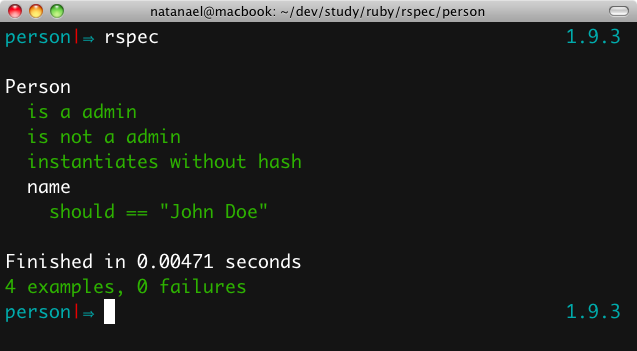
\includegraphics[width=0.65 \textwidth]{figuras/figura_31}
    \caption{Exemplo da DSL do RSpec}
    \label{figura_31}
\end{figure}

O resultado de execução do código acima pode ser visto na Figura \ref{figura_32}, a qual descreve os testes que passaram.

\begin{figure}[ht]
    \centering
    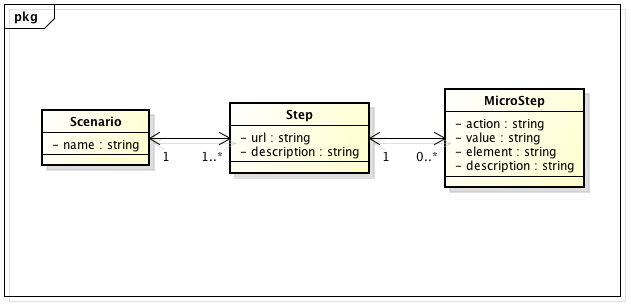
\includegraphics[width=0.6 \textwidth]{figuras/figura_32}
    \caption{Saída após rodar os testes com RSpec}
    \label{figura_32}
\end{figure}

Além da utilização desta biblioteca de testes, foi utilizado o conceito de "passos de bebê", ou seja, pequenas partes são desenvolvidas a cada momento, seja levantamento de requisitos, implementação de funcionalidade, refatoração ou até especificações. Um exemplo disto é focar no desenvolvimento de uma pequena parte de uma funcionalidade, diminuindo o risco do desenvolvimento e asegurando o atingimento de objetivos alcançaveis (RODRIGO, 2010).

\subsection{Testes desenvolvidos}

Todo processo de desenvolvimento da ferramenta utilizou TDD, onde foram criadas verificações unitárias dos models, views e controllers.

Os testes de model têm a responsabilidade de especificar e verificar a lógica de negócio da aplicação, avaliando o comportamento dos objetos. A figura \ref{figura_33} mostra uma parte do código do teste responsável pelo modelo Scenario.

\begin{figure}[htpb]
    \centering
    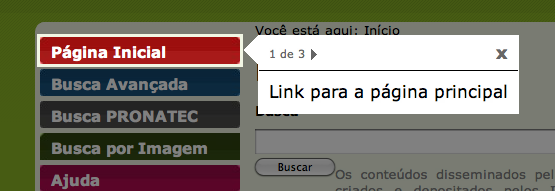
\includegraphics[width=0.7 \textwidth]{figuras/figura_33}
    \caption{Teste unitário do \textit{model}}
    \label{figura_33}
\end{figure}

A cobertura de testes atumatizados das views foram desenvolvidas para verificar se o conteúdo é corretamente apresentado ao usuário na página (Figura \ref{figura_34}).

\pagebreak

\begin{figure}[htpb]
    \centering
    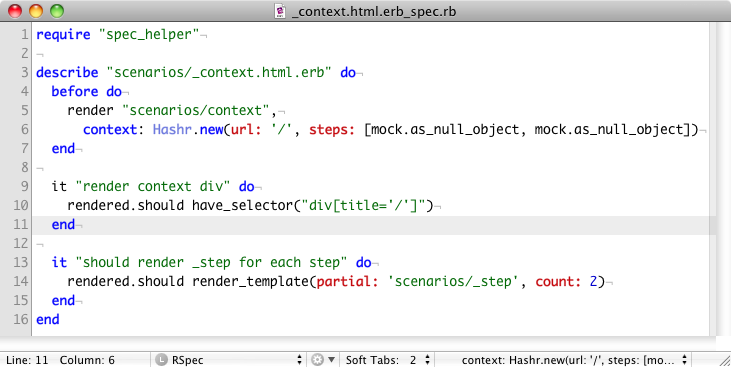
\includegraphics[width=0.7 \textwidth]{figuras/figura_34}
    \caption{Testes unitários da \textit{view}}
    \label{figura_34}
\end{figure}

No caso dos controllers, foram avaliados os comportamentos das classes controladoras da aplicação, as quais somente repassam requisições entre model e view (Figura \ref{figura_35}).

\begin{figure}[htpb]
    \centering
    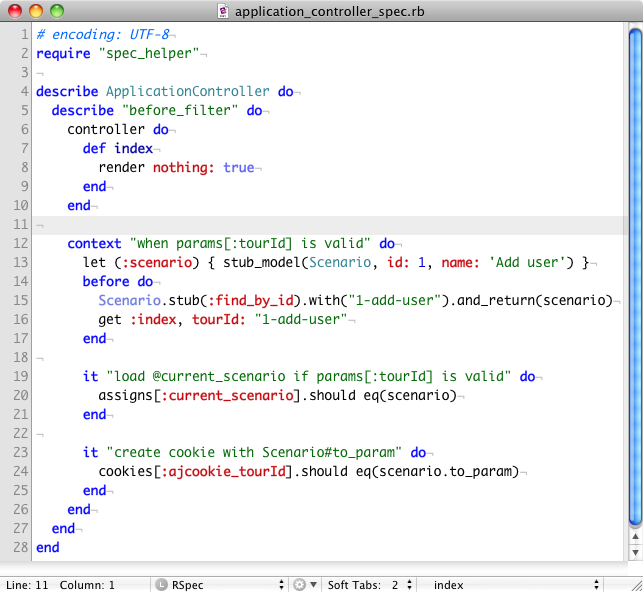
\includegraphics[width=0.7 \textwidth]{figuras/figura_35}
    \caption{Testes unitários do \textit{controller}}
    \label{figura_35}
\end{figure}

\subsection{Arquitetura da ferramenta}

O projeto inicial levou a construção de uma arquitetura onde os elementos constituintes da ferramenta se relacionavam conforme o modelo apresentado na Figura \ref{figura_36}.

\pagebreak

\begin{figure}[htpb]
    \centering
    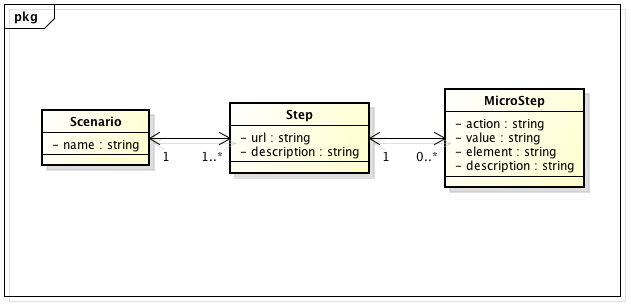
\includegraphics[width=0.7 \textwidth]{figuras/figura_36}
    \caption{Diagrama de classes da arquitetura inicial}
    \label{figura_36}
\end{figure}

Entretanto, após implementada esta arquitetura pode-se verificar a dificuldade na utilização da ferramenta. Foi então realizado um refatoramento que levou a descoberta de uma biblioteca da linguagem Ruby (Hashr) que facilitou uma nova arquitetura.

A biblioteca Hashr cria uma nova classe derivada da classe Hash, que simplifica o uso de hashes aninhados e acesso aos seus valores (GITHUB, 2012). A Figura \ref{figura_37} exemplifica o uso desta estrutura.

\begin{figure}[htpb]
    \centering
    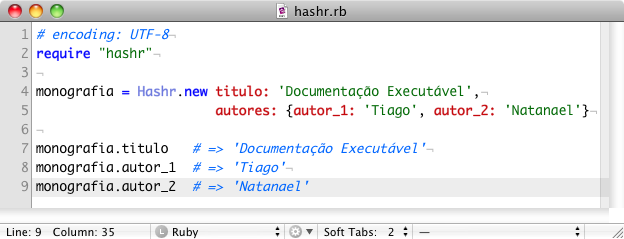
\includegraphics[width=0.8 \textwidth]{figuras/figura_37}
    \caption{Exemplo de uso do Hashr}
    \label{figura_37}
\end{figure}

Porém o exemplo acima não é a melhor representação da estrutura desejada. Os autores devem pertencer a uma lista, entretanto o Hashr não converte os itens da lista conforme esperado. Para resolver este problema, foi desenvolvido um método recursivo que converte os valores em lista produzindo assim os efeitos esperados.

\begin{figure}[htpb]
    \centering
    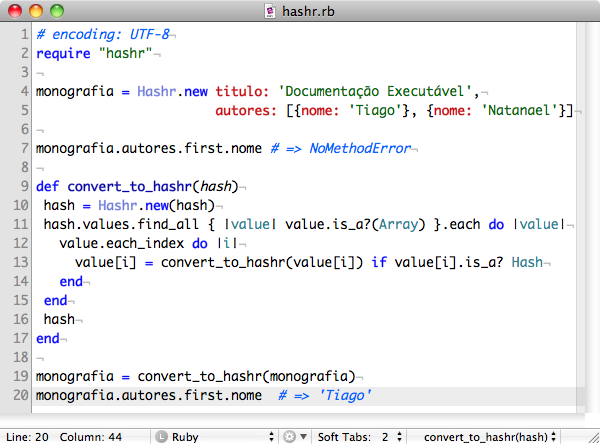
\includegraphics[width=0.7 \textwidth]{figuras/figura_38}
    \caption{Método de conversão de listas de Hash para Hashr}
    \label{figura_38}
\end{figure}
